\chapter{命令补充}

\section{打印系统相关的信息}
\begin{itemize}
\item 安装:
\begin{lstlisting}
# ubuntu 
$ sudo apt-get install -y screenfetch 
\end{lstlisting}

\item 运行:
\begin{lstlisting}
$ sudo screenfetch
\end{lstlisting}

% opensuse screenfetch  
% h: 当前位置(here)。将图形放置在正文文本中给出该图形环境的地方。如果本页所剩的页面不够,这一参数将不起作用。
% t: 顶部(top)。将图形放置在页面的顶部
% b: 底部(button)。将图形放置在页面的底部
% p: 独立一页(page)。将图形放置在一只允许有浮动对象的页面上。

\begin{figure}[htp]  
    \centering
    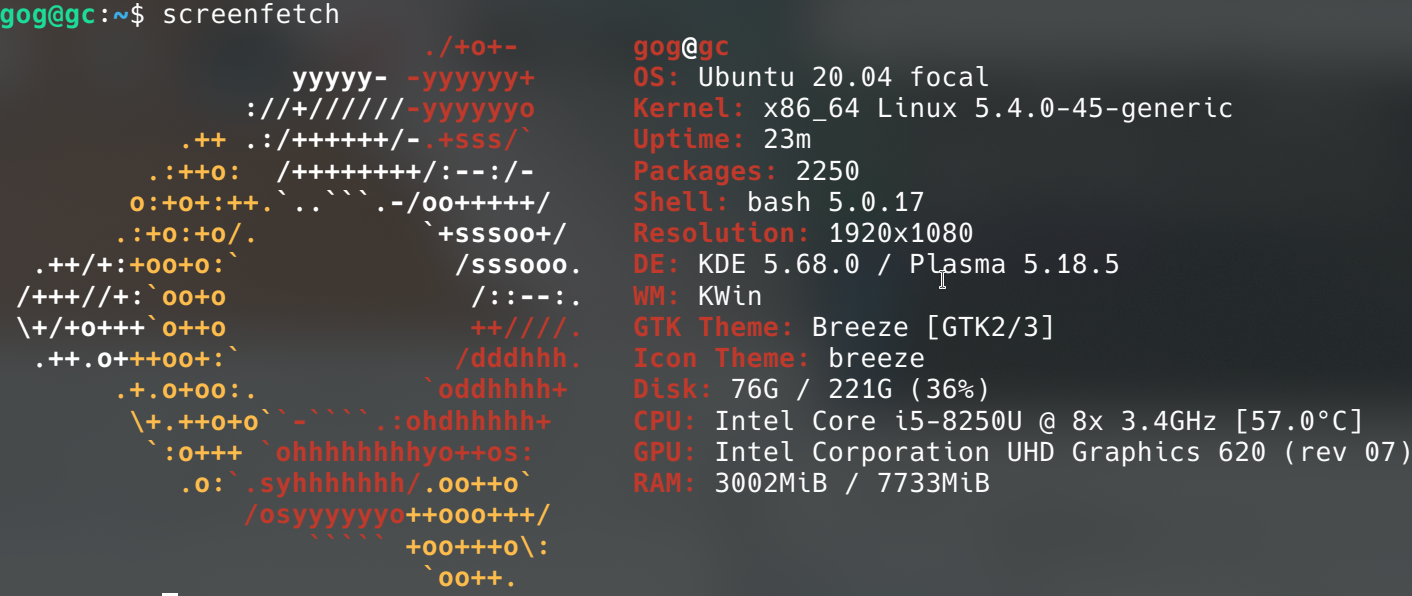
\includegraphics[width=0.49\textwidth]{./img/screenfetch/ubuntu.png}
    \caption{运行结果} %caption是图片的标题
    \label{fig:ubuntu_screenfetch} %此处的label相当于一个图片的专属标志,目的是方便上下文的引用
\end{figure}
\end{itemize}
\newpage

\section{apt}
debian 系\footnote{常见的 debian系:ubuntu, deepin, kubuntu, kail, xubuntu}用的最多的命令,是必需的命令之一。
\begin{itemize}
\item 常用命令
\begin{lstlisting}
# 更新软件列表
$ sudo apt-get update 

# 升级软件
$ sudo apt-get updrade 

# 删除包
$ sudo apt-get remove <package_name>

# 自动卸载软件,及其有依赖相关的软件包
$ sudo apt-get autoremove 

# 安装包
$ sudo apt-get install -y <package_name>

# 支持模糊搜索  
$ sudo apt-get search <package_name> 

# 解决依赖
$ sudo apt install -f
\end{lstlisting}


\item ppa 源\footnote{官网:https://launchpad.net/}
\newpage
	
\section{snap}
你可以通过\href{https://snapcraft.io/}{snap 应用商店}来查找软件,也可以通过命令行来查找。

\item 常用命令

snap 是一个包管理器,类似于 apt 可用于软件的安装、查找、卸载
\begin{lstlisting}
$ snap help 
$ snap search <包名> // 模糊查找
$ snap install <包名>
$ snap remove <包名>
$ snap list 
\end{lstlisting}

\item 例子:安装 vscode 
\begin{lstlisting}
$ snap install code
\end{lstlisting}
\end{itemize}

